\TNSA
\Opensolutionfile{ans}[ans/ans-2C5B3CD3-D1-KQ]
\begin{ex}%[2H5H3-2] 
	Cho mặt cầu $\left(S\right)$ có phương trình $(S)\colon\left( x-3 \right)^2+\left( y+2 \right)^2+\left( z-1 \right)^2=100$ và mặt phẳng $\left(\alpha\right)$ có	phương trình $2x-2y-z+9=0$. Tính bán kính của đường tròn là giao tuyến của mặt phẳng $\left(\alpha\right)$ và
	mặt cầu $\left(S\right)$.
	\shortans{$8$}
	\loigiai{
		\immini{	Gọi $I$ là tâm mặt cầu $(S)$, $H$ là hình chiếu vuông góc của $I$ lên mặt phẳng $(\alpha)$ và $AB$ là một đường kính của đường tròn $(C)$.\\
			Dễ thấy $I(3 ;-2 ; 1)$, $IA=10$, I $H=\mathrm{d}(I,(\alpha))=6$.\\ Suy ra $HA=\sqrt{IA^2-IH^2}=8$.\\
			Vậy bán kính đường tròn $(C)$ bằng $8$.	}{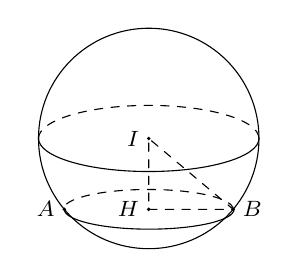
\begin{tikzpicture}[scale=0.7, font=\footnotesize,line join=round, line cap=round, >=stealth]
				\def\r{2}
				\def\a{1}
				\def\b{0.6}
				\pgfmathsetmacro\m{sin(40)}
				\pgfmathsetmacro\n{cos(40)}
				\path
				(0,0) coordinate (O)
				(\r*\n,-\r*\m) coordinate (M)
				(-\r*\n,-\r*\m) coordinate (N)
				(0,-\r*\m) coordinate (H)
				(0,\r) coordinate (A')
				(0,-\r) coordinate (A)
				;
				\draw	(O) circle (\r);
				\node at (O) [left] {$I$};
				\node at (M) [right] {$B$};
				\node at (N) [left] {$A$};
				\node at (H) [left] {$H$};
				%\node at (A') [above] {$A'$};
				%\node at (A) [below] {$A$};
				
				\fill (O) circle (1pt); 
				\fill (M) circle (1pt); 
				\fill (N) circle (1pt); 
				\fill (H) circle (1pt); 
				%\fill (A') circle (1pt); 
				%\fill (A) circle (1pt); 
				
				\draw	(180:\r) arc (180:360:{\r} and	{.3*\r});
				\draw[dashed]	(180:\r) arc (180:0:{\r} and	{.3*\r}) (H)--(M)--(O)--(H);
				
				\draw	(N) arc (180:360:{0.77*\r} and	{0.18*\r});
				\draw [dashed]	(M) arc (0:180:{0.77*\r} and	{0.18*\r});
		\end{tikzpicture}}
	}	
\end{ex}	

	\begin{ex}%[2H5H3-2] 
	Trong KG $Oxyz$, cho mặt phẳng $\left( P \right)\colon2x-y-2z-1=0$ và điểm $M\left( 1;-2;0 \right)$. Mặt cầu tâm $M$, bán kính bằng $\sqrt{3}$ cắt mặt phẳng $\left( P \right)$ theo giao tuyến là đường tròn có bán kính bằng bao nhiêu? (\textit{Kết quả làm tròn đến hàng phần trăm}).
	\shortans{$1{,}41$}
	\loigiai{
		\immini{	Mặt cầu tâm tâm $M$, bán kính bằng $R=\sqrt{3}$ cắt phẳng $\left( P \right)$ theo giao tuyến là đường tròn tâm $H$, bán kính $r$ suy ra $r=\sqrt{R^2-MH^2}$.\\
			Với $MH=\mathrm{d}\left( M,\left( P \right) \right)=\dfrac{\left| 2\cdot1-\left( -2 \right)-2\cdot0-1 \right|}{\sqrt{2^2+1^2+2^2}}=1$.\\
			Suy ra $r=\sqrt{{\left( \sqrt{3} \right)^2}-1^2}=\sqrt{2}\approx1{,}41$.}{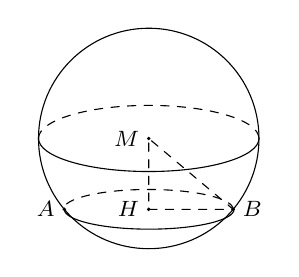
\begin{tikzpicture}[scale=0.7, font=\footnotesize,line join=round, line cap=round, >=stealth]
				\def\r{2}
				\def\a{1}
				\def\b{0.6}
				\pgfmathsetmacro\m{sin(40)}
				\pgfmathsetmacro\n{cos(40)}
				\path
				(0,0) coordinate (O)
				(\r*\n,-\r*\m) coordinate (M)
				(-\r*\n,-\r*\m) coordinate (N)
				(0,-\r*\m) coordinate (H)
				(0,\r) coordinate (A')
				(0,-\r) coordinate (A)
				;
				\draw	(O) circle (\r);
				\node at (O) [left] {$M$};
				\node at (M) [right] {$B$};
				\node at (N) [left] {$A$};
				\node at (H) [left] {$H$};
				%\node at (A') [above] {$A'$};
				%\node at (A) [below] {$A$};
				
				\fill (O) circle (1pt); 
				\fill (M) circle (1pt); 
				\fill (N) circle (1pt); 
				\fill (H) circle (1pt); 
				%\fill (A') circle (1pt); 
				%\fill (A) circle (1pt); 
				
				\draw	(180:\r) arc (180:360:{\r} and	{.3*\r});
				\draw[dashed]	(180:\r) arc (180:0:{\r} and	{.3*\r}) (H)--(M)--(O)--(H);
				
				\draw	(N) arc (180:360:{0.77*\r} and	{0.18*\r});
				\draw [dashed]	(M) arc (0:180:{0.77*\r} and	{0.18*\r});
		\end{tikzpicture}}
	}
\end{ex}

\begin{ex}%[2H5H3-2] 
	Trong không gian với hệ trục tọa độ $Oxyz$, cho mặt phẳng $(P)\colon2x+2y+z-m^2-3m=0$ và mặt cầu $(S)\colon\left( x-1 \right)^2+\left( y+1 \right)^2+\left( z-1 \right)^2=9$. Gọi $T$ là tập hợp tất cả các giá trị của $m$ để $(P)$ tiếp xúc với $(S)$. Tính tổng các phần tử của $T$.
	\shortans{$-3$}
	\loigiai{
		Ta có $(S)\colon\left\{ \begin{aligned}
			& I\left( 1;-1;1 \right) \\
			& R=3 \\
		\end{aligned} \right.$.\\
		$(P)$ tiếp xúc với $(S)$ khi và chỉ khi
		\begin{eqnarray*}
			& & d\left( I;\left( P \right) \right)=R\\
			&\Leftrightarrow & \dfrac{\left| 1-m^2-3m \right|}{3}=3\\
			&\Leftrightarrow & \left[ \begin{aligned}
				& {m^2}+3m-10=0 \\
				& {m^2}+3m+8=0 \\
			\end{aligned} \right.\\
			&\Leftrightarrow & \left[ \begin{aligned}
				& m=2 \\
				& m=-5 \\
			\end{aligned} \right.\\
		\end{eqnarray*}
	Vậy tổng các phần tử của $T$ là $-3$.
	}
\end{ex}

\begin{ex}%[2H5H3-2] 
	Trong không gian $\text{O}xyz$, cho mặt cầu $\left( S \right) \colon {{\left( x-2 \right)}^2}+{{\left( y-4 \right)}^2}+{{\left( z-1 \right)}^2}=4$ và mặt phẳng $\left( P \right): x+my+z-3m-1=0$. Gọi $T$ là tập hợp tất cả các giá trị của $m$ để mặt phẳng $\left( P \right)$ cắt mặt cầu $\left( S \right)$ theo giao tuyến là đường tròn có đường kính bằng $2$. Tính tổng các phần tử của $T$.
	\shortans{$1$}
	\loigiai{
	\immini{	Mặt cầu  $\left(S\right)\colon{{\left( x-2 \right)}^2}+{{\left( y-4 \right)}^2}+{{\left( z-1 \right)}^2}=4$ có tâm $I\left( 2;4;1 \right)$, bán kính $R=2$.\\
		Ta có $\mathrm{d}\left( I,\left( P \right) \right)=\dfrac{\left| 2+4m+1-3m-1 \right|}{\sqrt{1+m^2+1}}$ $=\dfrac{\left| m+2 \right|}{\sqrt{m^2+2}}$\\
		Mặt phẳng $\left( P \right)$ cắt mặt cầu $\left( S \right)$ theo giao tuyến là đường tròn có đường kính bằng $2$ nên bán kính đường tròn giao tuyến là $r=1$.}{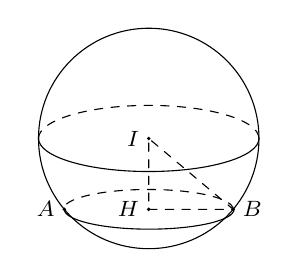
\begin{tikzpicture}[scale=0.7, font=\footnotesize,line join=round, line cap=round, >=stealth]
			\def\r{2}
			\def\a{1}
			\def\b{0.6}
			\pgfmathsetmacro\m{sin(40)}
			\pgfmathsetmacro\n{cos(40)}
			\path
			(0,0) coordinate (O)
			(\r*\n,-\r*\m) coordinate (M)
			(-\r*\n,-\r*\m) coordinate (N)
			(0,-\r*\m) coordinate (H)
			(0,\r) coordinate (A')
			(0,-\r) coordinate (A)
			;
			\draw	(O) circle (\r);
			\node at (O) [left] {$I$};
			\node at (M) [right] {$B$};
			\node at (N) [left] {$A$};
			\node at (H) [left] {$H$};
			%\node at (A') [above] {$A'$};
			%\node at (A) [below] {$A$};
			
			\fill (O) circle (1pt); 
			\fill (M) circle (1pt); 
			\fill (N) circle (1pt); 
			\fill (H) circle (1pt); 
			%\fill (A') circle (1pt); 
			%\fill (A) circle (1pt); 
			
			\draw	(180:\r) arc (180:360:{\r} and	{.3*\r});
			\draw[dashed]	(180:\r) arc (180:0:{\r} and	{.3*\r}) (H)--(M)--(O)--(H);
			
			\draw	(N) arc (180:360:{0.77*\r} and	{0.18*\r});
			\draw [dashed]	(M) arc (0:180:{0.77*\r} and	{0.18*\r});
	\end{tikzpicture}}
	
		Ta có 
		\begin{eqnarray*}
			& & R^2=d^2\left( I,\left( P \right) \right)+r^2\\
			&\Leftrightarrow & 4=\dfrac{{{\left( m+2 \right)}^2}}{m^2+2}+1\\
			&\Leftrightarrow & {m^2}+4m+4=3\left( {m^2}+2 \right)\\
				&\Leftrightarrow & 2m^2-4m+2=0\Leftrightarrow m=1.
		\end{eqnarray*}
	}
\end{ex}

\begin{ex}%[2H5H3-2] 
	Trong không gian với hệ trục toạ độ $Oxyz$, cho mặt cầu có phương trình $\left( S \right)\colon x^2+y^2+z^2+2x-4y-6z+m-3=0$. Gọi $T$ là tập hợp tất cả các giá trị của $m$ để mặt phẳng $\left( \beta \right)\colon2x-y+2z-8=0$ cắt $\left( S \right)$ theo một đường tròn có chu vi bằng $8\pi$. Tính tổng các phần tử của $T$.
	\shortans{$-1$}
	\loigiai{
		Ta có $\left( S \right)\colon x^2+y^2+z^2+2x-4y-6z+m-3=0\Leftrightarrow {{\left( x+1 \right)}^2}+{{\left( y-2 \right)}^2}+{{\left( z-3 \right)}^2}=17-m$.\\
		$\left( S \right)$ là phương trình của mặt cầu thì $17-m>0\Leftrightarrow m<17$.\\
		Khi đó $I\left( -1;2;3 \right);\ R=\sqrt{17-m}$ lần lượt là tâm và bán kính của $\left( S \right)$.\\
		Để mặt phẳng $\left( \beta \right)\colon2x-y+2z-8=0$ cắt $\left( S \right)$ theo thiết diện là một đường tròn có chu vi bằng $8\pi$ thì đường tròn đó có bán kính $r=4$.\\
		Ta có $R^2=d^2\left( I,\left( \beta \right) \right)+r^2\Leftrightarrow 17-m=16+2\Leftrightarrow m=-1$ (TMĐK).}
\end{ex}

\begin{ex}%[2H5H3-2] 
	Trong KG $Oxyz$ cho hai mặt phẳng $\left( P \right)\colon2x-y+z-2=0\,$ và $\left( Q \right)\colon2x-y+z+1=0$. Hỏi có bao nhiêu mặt cầu đi qua $A\left( 1;-2;1 \right)$ và tiếp xúc với hai mặt phẳng $\left( P \right)$, $\left( Q \right)$?
	\shortans{$0$}
	\loigiai{
		Ta có $\left(P\right)\parallel \left(Q\right)$, $M\left( 0;0;2 \right)\in \left( P \right)\Rightarrow \mathrm{d}\left( \left( P \right),\left( Q \right) \right)=\mathrm{d}\left( M,\left( Q \right) \right)=\dfrac{\sqrt{6}}{2}$\\
		$\mathrm{d}\left( A,\left( P \right) \right)=\dfrac{\sqrt{6}}{2}$; $\mathrm{d}\left( A,\left( Q \right) \right)=\sqrt{6}\Rightarrow \mathrm{d}\left( A,\left( Q \right) \right)=\mathrm{d}\left( A,\left( P \right) \right)+\mathrm{d}\left( \left( Q \right),\left( P \right) \right)$.\\
		Vậy không có mặt cầu thỏa yêu cầu bài toán.
	}
\end{ex}

\begin{ex}%[2H5H3-2]% Cau 6
	Trong KG $Oxyz$, cho mặt cầu $\left( S \right)\colon\left( x-1 \right)^2+\left( y-1 \right)^2+z^2=4$ và một điểm $M\left( 2;\,3;\,1 \right)$. Từ $M$ kẻ được vô số các tiếp tuyến tới $\left( S \right)$, biết tập hợp các tiếp điểm là đường tròn $\left( C \right)$. Tính bán kính $r$ của đường tròn $\left( C \right)$. (\textit{Kết quả làm tròn tới hàng phần trăm}).
	\shortans{$1{,}15$}
	\loigiai{
		\immini{	Mặt cầu $\left( S \right)$ có tâm $I\left( 1;1;0 \right)$ và bán kính $R=2$.\\
			Ta có $\overrightarrow{IM}=\left( 1;2;1 \right)$ và $IM=\sqrt{6}$.\\
			Gọi $H$ là một tiếp điểm tùy ý khi kẻ tiếp tuyến từ $M$ đến mặt cầu, khi đó $MH=\sqrt{IM^2-R^2}=\sqrt{2}$. Gọi $O$ là tâm của đường tròn $\left( C \right)$ khi đó $IM\bot HO$ và $HO=r$.\\
			Ta có $HI\cdot HM=HO\cdot IM\Rightarrow r=\dfrac{HI\cdot HM}{IM}=\dfrac{2\sqrt{2}}{\sqrt{6}}=\dfrac{2\sqrt{3}}{3}$.}{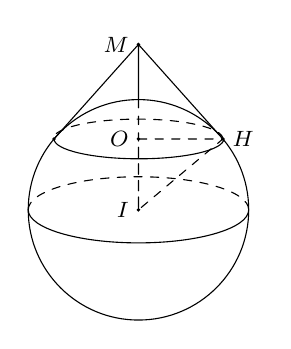
\begin{tikzpicture}[scale=0.7, font=\footnotesize,line join=round, line cap=round, >=stealth]
				\def\r{2}
				\def\a{1}
				\def\b{0.6}
				\pgfmathsetmacro\m{sin(40)}
				\pgfmathsetmacro\n{cos(40)}
				\path
				(0,0) coordinate (O)
				(0,3) coordinate (T)
				(\r*\n,\r*\m) coordinate (M)
				(-\r*\n,\r*\m) coordinate (N)
				(0,\r*\m) coordinate (H)
				(0,\r) coordinate (A')
				(0,-\r) coordinate (A)
				;
				\draw	(O) circle (\r);
				\node at (O) [left] {$I$};
				\node at (M) [right] {$H$};
				%\node at (N) [left] {$A$};
				\node at (H) [left] {$O$};
				\node at (T) [left] {$M$};
				%\node at (A') [above] {$A'$};
				%\node at (A) [below] {$A$};
				
				\fill (O) circle (1pt); 
				\fill (M) circle (1pt); 
				\fill (N) circle (1pt); 
				\fill (H) circle (1pt); 
				\fill (T) circle (1pt); 
				%\fill (A') circle (1pt); 
				%\fill (A) circle (1pt); 
				
				\draw	(180:\r) arc (180:360:{\r} and	{.3*\r}) (T)--(A') (T)--(M) (T)--(N);
				\draw[dashed]	(180:\r) arc (180:0:{\r} and	{.3*\r}) (H)--(M)--(O)--(H) (A')--(O);
				
				\draw	(N) arc (180:360:{0.77*\r} and	{0.18*\r});
				\draw [dashed]	(M) arc (0:180:{0.77*\r} and	{0.18*\r});
		\end{tikzpicture}}
	}
\end{ex}

\begin{ex}%[2H5H3-2] 
	Trong KG $Oxyz$, xét các điểm $A\left( 0;0;1 \right)$, $B\left( m;0;0 \right)$, $C\left( 0;n;0 \right)$, $D\left( 1;1;1 \right)$ với $m>0$; $n>0$ và $m+n=1$. Biết rằng khi $m$, $n$ thay đổi, tồn tại một mặt cầu cố định tiếp xúc với mặt phẳng $\left( ABC \right)$ và đi qua $D$. Tính bán kính $R$ của mặt cầu đó.
	\shortans{$1$}
	\loigiai{		
		Gọi $I\left( 1;1;0 \right)$ là hình chiếu vuông góc của $D$ lên mặt phẳng $(Oxy)$.\\
		Ta có phương trình theo đoạn chắn của mặt phẳng $(ABC)$ là $\dfrac{x}{m}+\dfrac{y}{n}+z=1$.\\
		Suy ra phương trình tổng quát của $(ABC)$ là $nx+my+mnz-mn=0$.\\
		Mặt khác $\mathrm{d}\left( I;\left( ABC \right) \right)=\dfrac{\left| 1-mn \right|}{\sqrt{m^2+n^2+m^2{n^2}}}=1$ (vì $m+n=1$)\\ và $ID=1=d(\left( I, \left( ABC \right) \right).$\\
		Nên tồn tại mặt cầu tâm $I$ (là hình chiếu vuông góc của $D$ lên mặt phẳng $Oxy$) tiếp xúc với $(ABC)$ và đi qua $D$. Khi đó $R=1$.}
\end{ex}
\Closesolutionfile{ans}
% \indapan{6}{ans/ans-2C5B3CD3-D1-KQ}
\begin{dang}
	{LẬP PHƯƠNG TRÌNH MẶT CẦU LIÊN QUAN ĐẾN MẶT PHẲNG}
\end{dang}
\TN
\Opensolutionfile{ans}[ans/ans-2C5B3CD3-D2]
\begin{ex}%[2H5H3-2] 
	Trong KG $Oxyz$, viết phương trình mặt cầu có tâm $I\left( 2;1;-4 \right)$ và tiếp xúc với mặt phẳng $\left( \alpha \right)\colon x-2y+2z-7=0$.
	\choice
	{$x^2+y^2+z^2+4x+2y-8z-4=0$}
	{$x^2+y^2+z^2+4x-2y+8z-4=0$}
	{\True $x^2+y^2+z^2-4x-2y+8z-4=0$}
	{$x^2+y^2+z^2-4x-2y-8z-4=0$}
	\loigiai{
		Mặt cầu cần tìm có bán kính $R=\mathrm{d}\left( I,\left( \alpha \right) \right)=\dfrac{\left| 2-2\cdot1+2\cdot\left( -4 \right)-7 \right|}{\sqrt{1^2+{\left( -2 \right)^2}+2^2}}=5$.\\
		Phương trình mặt cầu cần tìm là ${{\left( x-2 \right)}^2}+{{\left( y-1 \right)}^2}+{{\left( z+4 \right)}^2}=25$\\
		$\Leftrightarrow {x^2}+y^2+z^2-4x-2y+8z-4=0$.}
\end{ex}

\begin{ex}%[2H5H3-2] 
	Trong KG $Oxyz$, cho mặt cầu $\left( S \right)$ có tâm $I\left( 3;2;-1 \right)$ và đi qua điểm $A\left( 2;1;2 \right)$. Mặt phẳng nào dưới đây tiếp xúc với $\left( S \right)$ tại $A$?
	\choice
	{$x+y+3z-9=0$}
	{\True $x+y-3z+3=0$}
	{$x+y-3z-8=0$}
	{$x-y-3z+3=0$}
	\loigiai{
		Gọi $\left( P \right)$ là mặt phẳng cần tìm. Khi đó, $\left( P \right)$ tiếp xúc với $\left( S \right)$ tại $A$ khi chỉ khi $\left( P \right)$ đi qua $A\left( 2;1;2 \right)$ và nhận vectơ $\overrightarrow{IA}=\left( -1;-1;3 \right)$ làm vectơ pháp tuyến. Phương trình mặt phẳng $\left( P \right)$ là $-x-y+3z-3=0\Leftrightarrow x+y-3z+3=0$.}
\end{ex}

\begin{ex}%[2H5H3-2] 
	Trong KG $Oxyz$, cho mặt phẳng $\left( P \right)\colon x-2y+2z-2=0$ và điểm $I\left( -1;\,2;\,-1 \right)$. Viết phương trình mặt cầu $\left( S \right)$ có tâm $I$ và cắt mặt phẳng $\left( P \right)$ theo giao tuyến là đường tròn có bán kính bằng $5$.
	\choice
	{$\left( S \right)\colon\left( x+1 \right)^2+\left( y-2 \right)^2+\left( z+1 \right)^2=25$}
	{$\left( S \right)\colon\left( x+1 \right)^2+\left( y-2 \right)^2+\left( z+1 \right)^2=16$}
	{$\left( S \right)\colon\left( x-1 \right)^2+\left( y+2 \right)^2+\left( z-1 \right)^2=34$}
	{\True $\left( S \right)\colon\left( x+1 \right)^2+\left( y-2 \right)^2+\left( z+1 \right)^2=34$}
	\loigiai{
		Gọi $h$ là khoảng cách từ tâm $I$ đến mặt phẳng $\left( P \right)$ ta có:\\
		$h=\mathrm{d}\left( I;\left( P \right) \right)=\dfrac{\left| -1-4-2-2 \right|}{\sqrt{1^2+{{\left( -2 \right)}^2}+2^2}}=3$.\\
		Bán kính mặt cầu $\left( S \right)$ là $R=\sqrt{r^2+h^2}=\sqrt{5^2+3^2}=\sqrt{34}$.\\
		Phương trình mặt cầu $\left( S \right)$ là $\left( x+1 \right)^2+\left( y-2 \right)^2+\left( z+1 \right)^2=34$.}
\end{ex}

\begin{ex}%[2H5H3-3] 
	Trong KG $Oxyz$, mặt cầu $\left( S \right)$ có tâm $I\left( -1;\,2;\,1 \right)$ và tiếp xúc với mặt phẳng $\left( P \right)\colon x-2y-2z-2=0$ có phương trình là
	\choice
	{$\left( x+1 \right)^2+\left( y-2 \right)^2+\left( z-1 \right)^2=3$}
	{$\left( x-1 \right)^2+\left( y+2 \right)^2+\left( z+1 \right)^2=9$}
	{\True $\left( x+1 \right)^2+\left( y-2 \right)^2+\left( z-1 \right)^2=9$}
	{$\left( x+1 \right)^2+\left( y-2 \right)^2+\left( z+1 \right)^2=3$}
	\loigiai{
		Vì mặt cầu tâm $I\left( -1;\,2;\,1 \right)$ tiếp xúc với mặt phẳng $\left( P \right)\colon x-2y-2z-2=0$ nên bán kính\\
		$R=\mathrm{d}\left( I,\,\left( P \right) \right)=\dfrac{\left| -1-2\cdot2-2\cdot1-2 \right|}{\sqrt{1^2+\left( -2 \right)^2+\left( -2 \right)^2}}=3$ $\Rightarrow \left( S \right)\colon\left( x+1 \right)^2+\left( y-2 \right)^2+\left( z-1 \right)^2=9$.}
\end{ex}

\begin{ex}%[2H5H3-3] 
	Trong KG $Oxyz$, cho mặt cầu $\left( S \right)$ có tâm $I\left( 1;2;1 \right)$ và cắt mặt phẳng $\left( P \right)\colon2x-y+2z+7=0$ theo một đường tròn có đường kính bằng $8$. Phương trình mặt cầu $\left( S \right)$ là
	\choice
	{$\left( x-1 \right)^2+\left( y-2 \right)^2+\left( z-1 \right)^2=81$}
	{${{\left( x-1 \right)}^2}+{{\left( y-2 \right)}^2}+{{\left( z-1 \right)}^2}=5$}
	{${{\left( x+1 \right)}^2}+{{\left( y+2 \right)}^2}+{{\left( z+1 \right)}^2}=9$}
	{\True ${{\left( x-1 \right)}^2}+{{\left( y-2 \right)}^2}+{{\left( z-1 \right)}^2}=25$}
	\loigiai{
	
		Khoảng cách từ tâm $I$ đến mặt phẳng $\left( P \right)$ là\\
		$d=\mathrm{d}\left( I,\left( P \right) \right)=\dfrac{\left| 2\cdot1-2+2\cdot1+7 \right|}{\sqrt{2^2+{{\left( -1 \right)}^2}+2^2}}=3$.\\
		Đường tròn giao tuyến có đường kính bằng $8$ nên bán kính đường tròn là $r=4$.\\
		Bán kính của mặt cầu $\left( S \right)$là $R=\sqrt{d^2+r^2}=\sqrt{3^2+4^2}=5$.\\
		Vậy phương trình mặt cầu $\left( S \right)$ là ${{\left( x-1 \right)}^2}+{{\left( y-2 \right)}^2}+{{\left( z-1 \right)}^2}=25$.}
\end{ex}

\begin{ex}%[2H5H3-2] 
	Trong không gian với hệ trục toạ độ $Oxyz$, phương trình nào dưới đây là phương trình của mặt cầu có tâm $I\left( 3;1;0 \right)$ và tiếp xúc với mặt phẳng $\left( P \right): 2x + 2y - z + 1=0$?
	\choice
	{${{\left( x+3 \right)}^2}+{{\left( y+1 \right)}^2}+z^2=3$}
	{${{\left( x+3 \right)}^2}+{{\left( y+1 \right)}^2}+z^2=9$}
	{${{\left( x-3 \right)}^2}+{{\left( y-1 \right)}^2}+z^2=3$}
	{\True ${{\left( x-3 \right)}^2}+{{\left( y-1 \right)}^2}+z^2=9$}
	\loigiai{
		Gọi $\left( S \right)$ là mặt cầu có tâm $I$và tiếp xúc với $\left( P \right)$ có $R$ là bán kính.\\
		 Khi đó ta có $\mathrm{d}\left( I,\left( P \right) \right)=R\Rightarrow R=\dfrac{\left| 2\cdot3+2\cdot1-0+1 \right|}{\sqrt{2^2+2^2+{{\left( -1 \right)}^2}}}\Leftrightarrow R=3$.\\
		Vậy phương trình của $\left( S \right)$ là ${{\left( x-3 \right)}^2}+{{\left( y-1 \right)}^2}+z^2=9$.}
\end{ex}

\begin{ex}%[2H5H3-2] 
	Trong KG $Oxyz$, cho mặt cầu $\left( S \right)$ có tâm $I\left( 2;1;1 \right)$ và mặt phẳng $\left( P \right)\colon2x+y+2z+2=0$. Biết mặt phẳng $\left( P \right)$ cắt mặt cầu $\left( S \right)$ theo giao tuyến là một đường tròn có bán kính bằng $1$. Viết phương trình của mặt cầu $\left( S \right)$.
	\choice
	{$\left( S \right)\colon\left( x+2 \right)^2+\left( y+1 \right)^2+\left( z+1 \right)^2=8$}
	{$\left( S \right)\colon\left( x+2 \right)^2+\left( y+1 \right)^2+\left( z+1 \right)^2=10$}
	{$\left( S \right)\colon\left( x-2 \right)^2+\left( y-1 \right)^2+\left( z-1 \right)^2=8$}
	{\True $\left( S \right)\colon\left( x-2 \right)^2+\left( y-1 \right)^2+\left( z-1 \right)^2=10$}
	\loigiai{
		Gọi $R$, $r$ lần lượt là bán kính của mặt cầu $\left( S \right)$ và đường tròn giao tuyến\\
		Ta có ${R^2=r^2+{{\left( \mathrm{d}\left( I,\left( P \right) \right) \right)}^2}=1+{{\left( \dfrac{\left| 2\cdot2+1\cdot1+2\cdot1+2 \right|}{\sqrt{2^2+1+2^2}} \right)}^2}=10}$.\\
		Mặt cầu $\left( S \right)$ tâm $I\left( 2;1;1 \right)$ bán kính $R=\sqrt{10}$ là ${{\left( x-2 \right)}^2}+{{\left( y-1 \right)}^2}+{{\left( z-1 \right)}^2}=10$}
\end{ex}

\begin{ex}%[2H5H3-2] 
	Trong không gian với hệ trục tọa độ $Oxyz$, phương trình nào dưới đây là phương trình mặt cầu đi qua ba điểm $M\left( 2;3;3 \right)$, $N\left( 2;-1;-1 \right)$, $P\left( -2;-1;3 \right)$ và có tâm thuộc mặt phẳng $\left( \alpha \right)\colon2x+3y-z+2=0$?
	\choice
	{$x^2+y^2+z^2+4x-2y+6z+2=0$}
	{$x^2+y^2+z^2-2x+2y-2z-2=0$}
	{$x^2+y^2+z^2-2x+2y-2z-10=0$}
	{\True $x^2+y^2+z^2-4x+2y-6z-2=0$}
	\loigiai{
		Giả sử phương trình mặt cầu $\left( S \right)$ có dạng $x^2+y^2+z^2-2ax-2by-2cz+d=0$.\\
		Điều kiện: $a^2+b^2+c^2-d>0$ \hfill(*) \\
		Vì mặt cầu $\left( S \right)$ đi qua 3 điểm $M\left( 2;3;3 \right)$, $N\left( 2;-1;-1 \right)$, $P\left( -2;-1;3 \right)$ và có tâm $I$ thuộc $mp\left( P \right)$ nên ta có hệ phương trình\\ $\left\{ \begin{aligned}
			& 4a+6b+6c-d=22 \\
			& 4a-2b-2c-d=6 \\
			& 4a+2b-6c+d=-14 \\
			& 2a+3b-c=-2 \\
		\end{aligned} \right.\Leftrightarrow \left\{ \begin{aligned}
			& a=2 \\
			& b=-1 \\
			& c=3 \\
			& d=-2 \\
		\end{aligned} \right.\,\,(\text{thỏa mãn}\left( * \right))$\\
		Vậy phương trình mặt cầu là $x^2+y^2+z^2-4x+2y-6z-2=0.$}
\end{ex}

\begin{ex}%[2H5H3-2] 
	Trong KG $Oxyz$, cho điểm $I(-3;0;1)$. Mặt cầu $(S)$ có tâm $I$ và cắt mặt phẳng $(P)\colon x-2y-2z-1=0$ theo một thiết diện là một hình tròn. Diện tích của hình tròn này bằng $\pi$. Phương trình mặt cầu $(S)$ là
	\choice
	{$(x+3)^2+y^2+(z-1)^2=4$}
	{$(x+3)^2+y^2+(z-1)^2=25$}
	{\True $(x+3)^2+y^2+(z-1)^2=5$}
	{$(x+3)^2+y^2+(z-1)^2=2$}
	\loigiai{
		Gọi $S$, $r$ lần lượt là diện tích hình tròn và bán kính hình tròn.\\
		Ta có $S=\pi r^2=\pi \Rightarrow r=1$.\\
		$\mathrm{d}\left( I, \left( P \right) \right)=\dfrac{\left| -3-2\cdot0-2\cdot1-1 \right|}{\sqrt{1+4+4}}=2$.\\
		$(S)$ có tâm $I(-3;0;1)$ và bán kính $R=\sqrt{\left(\mathrm{d}\left( I,\left( P \right)\right) \right)^2+r^2}=\sqrt{2^2+1^2}=\sqrt{5}$.\\
		Phương trình mặt cầu $(S)$ là $(x+3)^2+y^2+(z-1)^2=5$.}
\end{ex}

\begin{ex}%[2H5H3-2] 
	Trong KG $Oxyz$, cho mặt phẳng $\left( P \right)\colon x-2y+2z-2=0$ và điểm $I\left( -1\,;\,\,2\,;\,\,-1 \right)$. Viết phương trình mặt cầu $\left( S \right)$ có tâm $I$ và cắt mặt phẳng $\left( P \right)$ theo giao tuyến là đường tròn có bán kính bằng $5$.
	\choice
	{$\left( S \right)\colon\left( x+1 \right)^2+\left( y-2 \right)^2+\left( z+1 \right)^2=25$}
	{$\left( S \right)\colon\left( x+1 \right)^2+\left( y-2 \right)^2+\left( z+1 \right)^2=16$}
	{$\left( S \right)\colon\left( x-1 \right)^2+\left( y+2 \right)^2+\left( z-1 \right)^2=34$}
	{\True $\left( S \right)\colon\left( x+1 \right)^2+\left( y-2 \right)^2+\left( z+1 \right)^2=34$}
	\loigiai{
		Gọi $M$ là điểm nằm trên đường tròn giao tuyến của $\left( S \right)$ và $\left( P \right)$. Ta có $IM=R$. Áp dụng công thức tính bán kính mặt cầu trong trường hợp mặt cầu $\left( S \right)$ giao với mặt phẳng $\left( P \right)$ theo giao tuyến là đường tròn có bán kính $r$ là\\
		$IM^2=R^2=d^2\left( I\,,\,\left( P \right) \right)+r^2$ \hfill(*)\\
		Ta có ${\mathrm{d}\left( I,\left( P \right) \right)}=\dfrac{\left| -1-2\cdot2+2\cdot\left( -1 \right)-2 \right|}{\sqrt{1^2+{{\left( -2 \right)}^2}+2^2}}=3=IH$.\\
		Từ $\left( * \right)\Rightarrow {R^2}=3^2+5^2=34$.\\
		Vậy phương trình mặt cầu $\left( S \right)$ thỏa mãn yêu cầu đề bài là\\ ${{\left( x+1 \right)}^2}+{{\left( y-2 \right)}^2}+{{\left( z+1 \right)}^2}=34$.}
\end{ex}
\Closesolutionfile{ans}
% \indapan{10}{ans/ans-2C5B3CD3-D2}
\TNSA
\Opensolutionfile{ans}[ans/ans-2C5B3CD3-D2-KQ]
\begin{ex}%[2H5H3-2] 
	Trong KG $Oxyz$, cho điểm $A\left( 1;2;3 \right)$. Tính bán kính của mặt cầu tâm $A$ và tiếp xúc với mặt phẳng $x-2y+2z+3=0$.
		\shortans{$2$}
	\loigiai{
		${{\left( x-1 \right)}^2}+{{\left( y-2 \right)}^2}+{{\left( z-3 \right)}^2}=4$\\
		Mặt cầu tâm $A$ tiếp xúc với mặt phẳng đã cho có bán kính $R=\dfrac{\left| 1-2\cdot2+2\cdot3+3 \right|}{\sqrt{1+4+4}}=2$.}
\end{ex}

